% One outer step of meta-training, MAML against Meta-LSQ (one column). Hand-written TikZ, 16 Nov 2026.
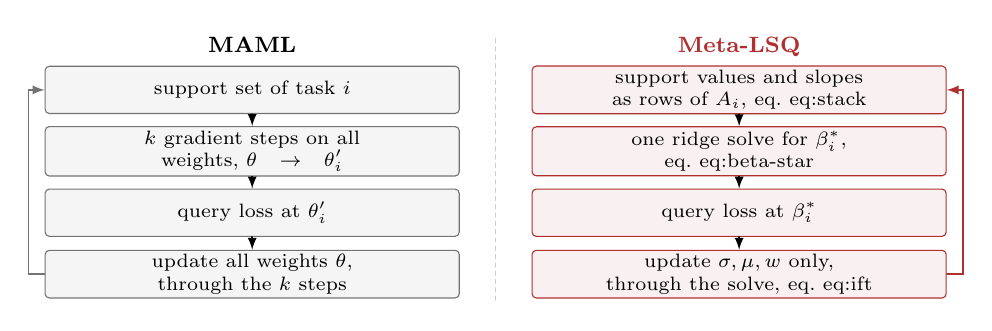
\begin{tikzpicture}[x=\linewidth, y=1cm, line cap=round,
    box/.style={draw=black!55, fill=black!4, rounded corners=1.5pt, line width=0.4pt,
                align=center, text width=0.425\linewidth, inner sep=1.5pt, minimum height=0.6cm,
                font=\scriptsize},
    lsq/.style={box, draw=wfred, fill=wfred!7},
    arr/.style={-latex, line width=0.5pt}]
\definecolor{wfred}{HTML}{B03030}
\node[font=\footnotesize\bfseries, anchor=base] at (0.245, 0.48) {MAML};
\node[font=\footnotesize\bfseries, anchor=base, text=wfred] at (0.755, 0.48) {Meta-LSQ};
% MAML lane
\node[box] (m1) at (0.245, 0)     {support set of task $i$};
\node[box] (m2) at (0.245, -0.78) {$k$ gradient steps on all\\weights, $\theta \to \theta_i'$};
\node[box] (m3) at (0.245, -1.56) {query loss at $\theta_i'$};
\node[box] (m4) at (0.245, -2.34) {update all weights $\theta$,\\through the $k$ steps};
% Meta-LSQ lane
\node[lsq] (l1) at (0.755, 0)     {support values and slopes\\as rows of $A_i$, eq.~\eqref{eq:stack}};
\node[lsq] (l2) at (0.755, -0.78) {one ridge solve for $\beta_i^\ast$,\\eq.~\eqref{eq:beta-star}};
\node[lsq] (l3) at (0.755, -1.56) {query loss at $\beta_i^\ast$};
\node[lsq] (l4) at (0.755, -2.34) {update $\sigma, \mu, w$ only,\\through the solve, eq.~\eqref{eq:ift}};
\foreach \a/\b in {m1/m2, m2/m3, m3/m4, l1/l2, l2/l3, l3/l4} \draw[arr] (\a) -- (\b);
\draw[arr, black!55] (m4.west) -- ++(-0.017, 0) |- (m1.west);
\draw[arr, wfred] (l4.east) -- ++(0.017, 0) |- (l1.east);
\draw[black!20, line width=0.4pt, dash pattern=on 1.5pt off 1.5pt] (0.5, 0.65) -- (0.5, -2.7);
\end{tikzpicture}
